\usetikzlibrary{arrows.meta,shapes.misc}
\begin{frame}{timeouts per message} 
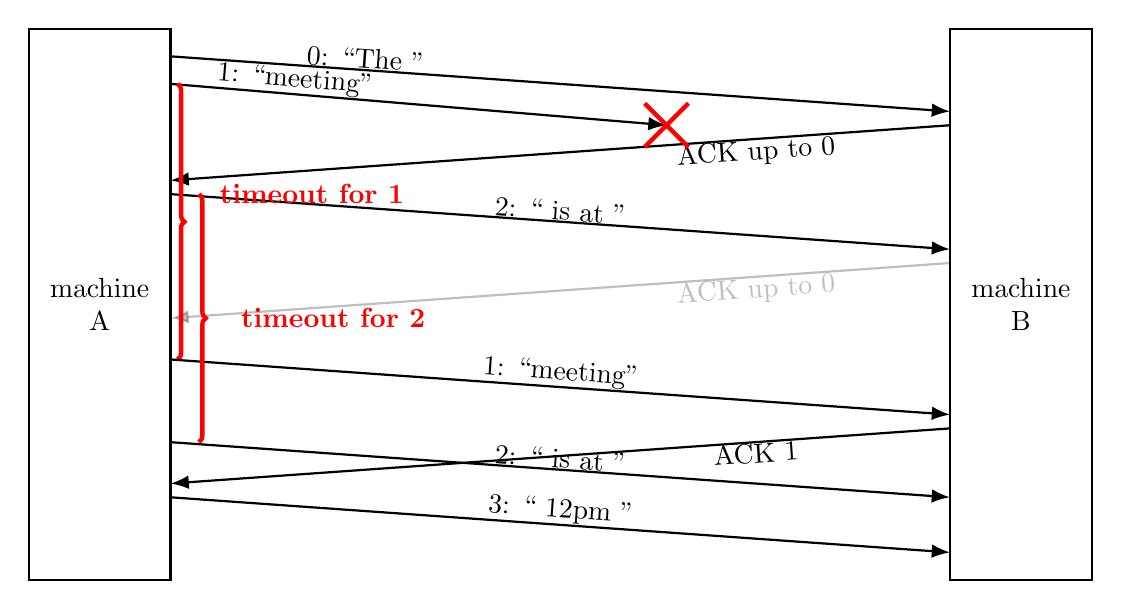
\begin{tikzpicture}
\tikzset{
    box/.style={thick},
    message/.style={draw,thick,-Latex},
    failure/.style={draw,ultra thick,red,cross out,minimum width=.5cm,minimum height=.5cm},
    every node/.style={inner sep=0.1mm},
}
\begin{scope}[xshift=1cm,x=0.9cm,y=0.7cm]
\draw[box] (0, 0) rectangle ++(2, -10) 
    node[midway,align=center] {machine\\A};
\draw[box] (13, 0) rectangle ++(2, -10) 
    node[midway,align=center] {machine\\B};
\draw[message] (2, -0.5) -- (13, -1.5) node[pos=0.25,above,sloped] {\myemph{0}: ``The ''};
\draw[message] (13, -1.75) -- (2, -2.75) node[pos=0.25,sloped,below] {ACK up to \myemph{0}};
\draw[message] (2, -1) -- (9, -1.75) node[pos=0.25, above, sloped] {\myemph{1}: ``meeting''}
    node[failure] {};
%\draw[message] (13, -2.25) -- (2, -3.25) node[pos=0.25, sloped,below] {got \myemph{1}};

% in response to got 0
\draw[message] (2, -3) -- (13, -4) node[pos=0.5, above, sloped] {\myemph{2}: `` is at ''};
%\draw[message] (13, -4.25) -- (2, -5.25) node[pos=0.25, sloped,below,alt=<2>{draw=red,ultra thick}] {ACK up to \myemph{0}};
\draw[message,opacity=0.25] (13, -4.25) -- (2, -5.25) node[pos=0.25, sloped,below] {ACK up to \myemph{0}};

\draw[ultra thick,red,decorate,decoration={brace}] (2.1, -1) -- (2.1, -6) node[pos=0.4,right=0.5cm] {\bfseries timeout for 1};
\draw[message] (2, -6) -- (13, -7) node[pos=0.5, above, sloped] {\myemph{1}: ``meeting''};
\draw[message] (13, -7.25) -- (2, -8.25) node[pos=0.25, sloped,below] {ACK \myemph{1}};
\draw[message] (2, -8.5) -- (13, -9.5) node[pos=0.5, above, sloped] {\myemph{3}: `` 12pm ''};

\draw[ultra thick,red,decorate,decoration={brace}] (2.4, -3) -- (2.4, -7.5) node[pos=0.5,right=0.5cm] {\bfseries timeout for 2};
\draw[message] (2, -7.5) -- (13, -8.5) node[pos=0.5, above, sloped] {\myemph{2}: `` is at ''};
\end{scope}
\end{tikzpicture}
\end{frame}
